\documentclass[xcolor=table]{beamer}

% for themes, etc.
\mode<presentation>
{  
	\setbeamertemplate{background canvas}[vertical shading][bottom=red!10,top=blue!10]
	\usetheme{Warsaw}
	\usefonttheme[onlysmall]{structurebold}
}

\usepackage{times}  % fonts are up to you
\usepackage{graphicx}
\usepackage{subfigure}
\definecolor{blue2}{cmyk}{.94,.11,0,0}
% these will be used later in the title page

\setbeamerfont{footnote}{size=\tiny}

\title[Distributed Processing Systems Presentation]{Copysets : Reducing the Frequency of Data Loss in Cloud Storage}
\author[Wei-Chih Chien]{Wei-Chih Chien\\ 60347046S}
\institute[NTNU CSIE LAB107]{NTNU CSIE LAB107}
\date{}

\AtBeginSection[]
{
  \begin{frame}<beamer>
    \frametitle{Outline}
    \tableofcontents[currentsection]
  \end{frame}
}

% have this if you'd like a recurring outline
\begin{document}

	% this prints title, author etc. info from above
	\begin{frame}
		\titlepage
	\end{frame}

	\begin{frame}
		\frametitle{Author \& Reference}
		Author:
		\begin{center}
			A. Cidon, S. Rumble, R. Stutsman,\\
			S. Katti, J. Ousterhout and M. Rosenblum\\
			(Standford University)
		\end{center}
		
		Source:
		\begin{center}
			2013 USENIX Annual Technical Conference\\
			(Awarded Best Student Paper)
		\end{center}
	
		\footnotetext[1]{www.usenix.org/conference/atc13/technical-sessions/presentation/cidon}
	\end{frame}

	\section{Introduction}

	\subsection{Random Replication}
	\begin{frame}
		\frametitle{Random Replication}
		\footnotesize
		Widely used in \underline{data center storage systems} to prevent data loss.
		\begin{itemize}
			\item Hadoop Distributed File System (HDFS)
			\item RAMCloud	     \textit{(https://ramcloud.stanford.edu)}
			\item Google File System (GFS)
			\item Windows Azure
		\end{itemize}
		However, large-scale correlated failures such as \alert{cluster power outages} handled poorly by random replication.$^\text{[1][2][3][4]}$\\
		This stresses the \alert{availability} of the system.
	
		\footnotetext[1]{R. J. Chansler. Data Availability and Durability with the Hadoop Distributed File System.}
		\footnotetext[2]{J. Dean. Evolution and future directions of large-scale storage and computation systems at Google.}
		\footnotetext[3]{D. Ford et al. Availability in globally distributed storage systems.}
		\footnotetext[4]{K. Shvachko et al. The hadoop distributed file system.}
	\end{frame}

	\subsection{Copysets Replication}
	\begin{frame}
		\frametitle{Copysets Replication}
		\begin{itemize}
			\item Split node into \alert{copysets}
			\item Replicas of single chunk can only be stored on \alert{one copyset}.
			\item Data loss events occur only when all the nodes of some copyset fail \alert{simultaneously}.
			\item \alert{Decrease} the probability of data loss under power outages.
		\end{itemize}
	\end{frame}

	\section{Intuition}

	\subsection{Probability of data loss}
	\begin{frame}
		\frametitle{Probability of data loss}
		\begin{minipage}[h]{0.49\linewidth}
			\centering
			\small
			\begin{itemize}
				\item N : \# nodes in the system
				\item R : \# replicas of each chunk
			\end{itemize}
		\end{minipage}
		\begin{minipage}[h]{0.49\linewidth}
			\centering
			\Huge
			$\frac{\# copyset}{\binom{N}{R}}$
		\end{minipage}
		\newline
		\newline
		Example :
		\begin{center}
			\alert{\{1, 2, 3\}, \{4, 5, 6\}, \{7, 8, 9\}}
			\newline
			\newline
			N = 9\newline
			R = 3
			\newline
			\newline
			\# copysets = 3
			\newline
		\end{center}
	\end{frame}

	\begin{frame}
		\begin{figure}[htb]
			\begin{minipage}[b]{0.49\linewidth}
				\centering
				\graphicspath{{fig/}}
				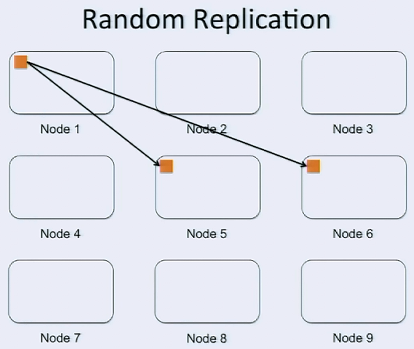
\includegraphics[width=1\textwidth]{1.png}
				\caption{1}
			\end{minipage}
			\begin{minipage}[b]{0.49\linewidth}
				\centering
				\graphicspath{{fig/}}
				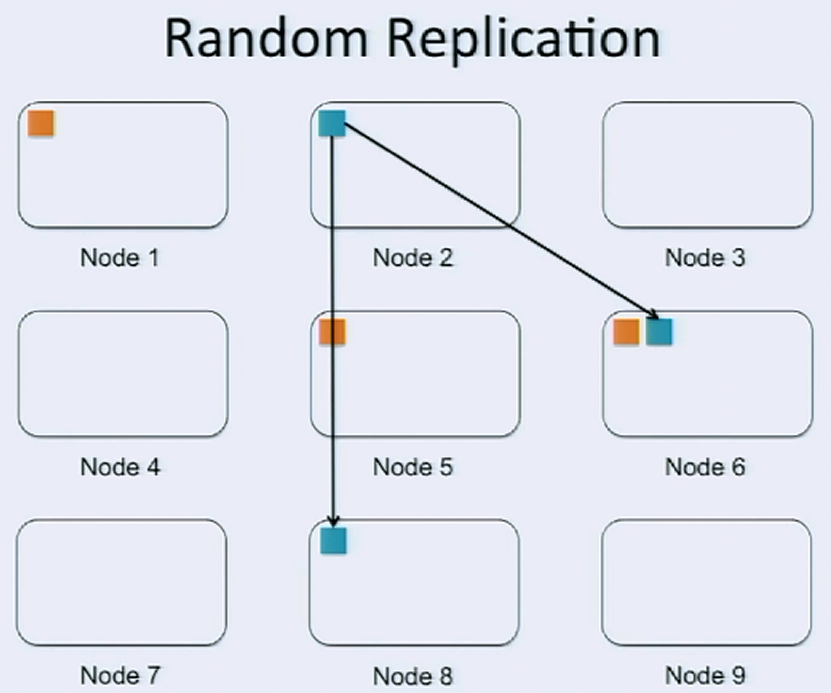
\includegraphics[width=1\textwidth]{2.png}
				\caption{2}
			\end{minipage}
		\end{figure}
	\end{frame}

	\begin{frame}
		\begin{figure}[htb]
			\begin{minipage}[b]{0.69\linewidth}
				\centering
				\graphicspath{{fig/}}
				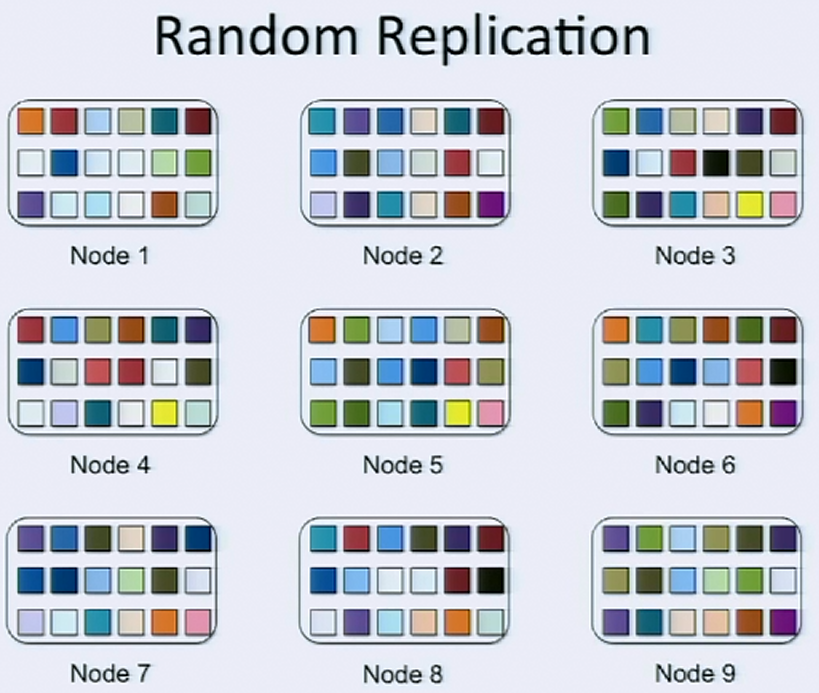
\includegraphics[width=1\textwidth]{3.png}
			\end{minipage}
			\begin{minipage}[b]{0.29\linewidth}
				\begin{center}
					\alert{	\{1, 5, 6\}\\
							\{2, 6, 8\}\\
							\{3, 4, 5\}\\
							...\\
							\{5, 6, 9\} }
				\end{center}
			\end{minipage}
		\end{figure}
	\end{frame}

	\begin{frame}
		\begin{figure}[htb]
			\begin{minipage}[b]{0.69\linewidth}
				\centering
				\graphicspath{{fig/}}
				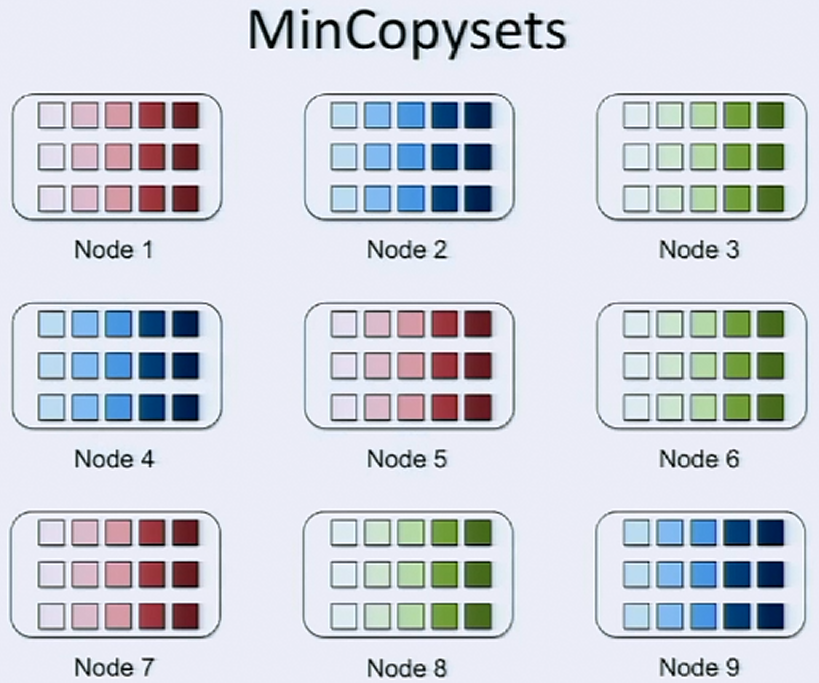
\includegraphics[width=1\textwidth]{4.png}
			\end{minipage}
			\begin{minipage}[b]{0.29\linewidth}
				\begin{center}
					\alert{	\{1, 5, 7\}\\
							\{2, 4, 9\}\\
							\{3, 6, 8\} }
				\end{center}
			\end{minipage}
		\end{figure}
	\end{frame}

	\begin{frame}
		\frametitle{Probability of data loss}
		\begin{minipage}[h]{0.49\linewidth}
			\centering
			\small
			\begin{itemize}
				\item N : \# nodes in the system
				\item R : \# replicas of each chunk
			\end{itemize}
		\end{minipage}
		\begin{minipage}[h]{0.49\linewidth}
			\centering
			\Huge
			$\frac{\# copyset}{\binom{N}{R}}$
		\end{minipage}
		\newline
		\newline
		Example :
		\begin{center}
			\alert{\{1, 2, 3\}, \{4, 5, 6\}, \{7, 8, 9\}}
			\newline
			\newline
			N = 9\newline
			R = 3
			\newline
			\newline
			\# copysets = 3
			\newline
		\end{center}
	\end{frame}

	\subsection{The Trade-off}
	\begin{frame}
		\frametitle{The Trade-off}
		% Please add the following required packages to your document preamble:
		% \usepackage[table,xcdraw]{xcolor}
		% If you use beamer only pass "xcolor=table" option, i.e. \documentclass[xcolor=table]{beamer}
		\begin{table}[h]
			\begin{tabular}{|c|c|c|}
				\hline
				\rowcolor[HTML]{3B9CF0} 
					& MinCopysets & Random Replication \\ \hline
				\rowcolor[HTML]{00D2CB} 
				Mean time to Failure & 625 years   & 1 year             \\ \hline
				\rowcolor[HTML]{00D2CB} 
				Amount of Data Lost  & 1 TB        & 5.5 GB             \\ \hline
			\end{tabular}
		\end{table}
		\begin{center}
			5000-node cluster
		\end{center}
	\end{frame}

	\section{Design}
	\begin{frame}
		\frametitle{Design}
		\begin{itemize}
			\small
			\item 2 phases : \alert{Permutation} \& \alert{Replication}.
			\item Scatter width : \# nodes that store copies for each node’s data.
		\end{itemize}
		\begin{figure}[htb]
			\begin{minipage}[b]{0.49\linewidth}
				\centering
				\graphicspath{{fig/}}
				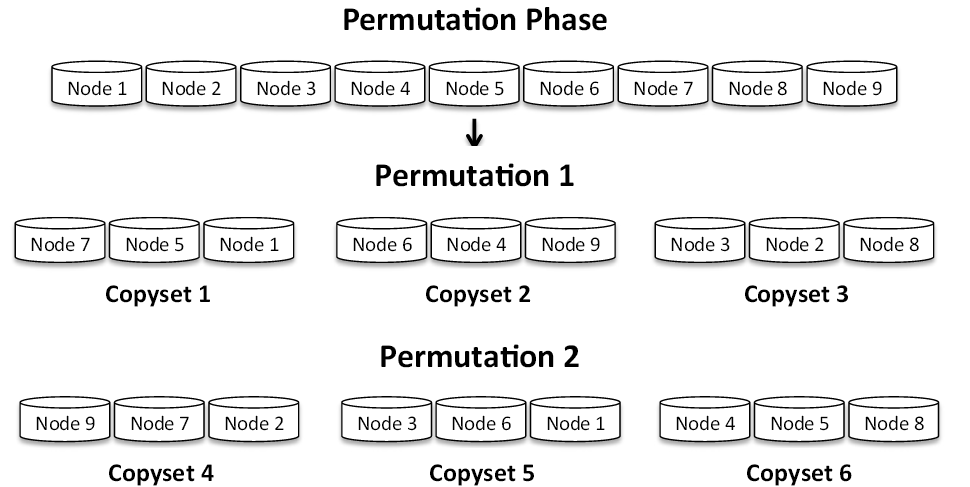
\includegraphics[width=1\textwidth]{5.png}
			\end{minipage}
			\begin{minipage}[b]{0.49\linewidth}
				\centering
				\graphicspath{{fig/}}
				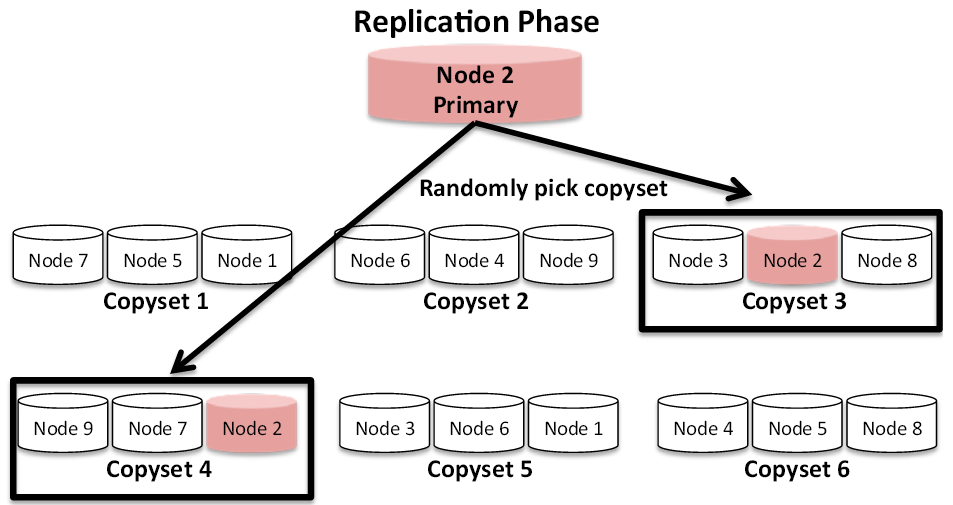
\includegraphics[width=1\textwidth]{6.png}
			\end{minipage}
		\end{figure}
	\end{frame}

	\begin{frame}
		\small
		\alert{Data loss probability} of \underline{random replication} and \underline{Copyset Replication} in different systems.
		\begin{figure}[htb]
			\centering
			\graphicspath{{fig/}}
			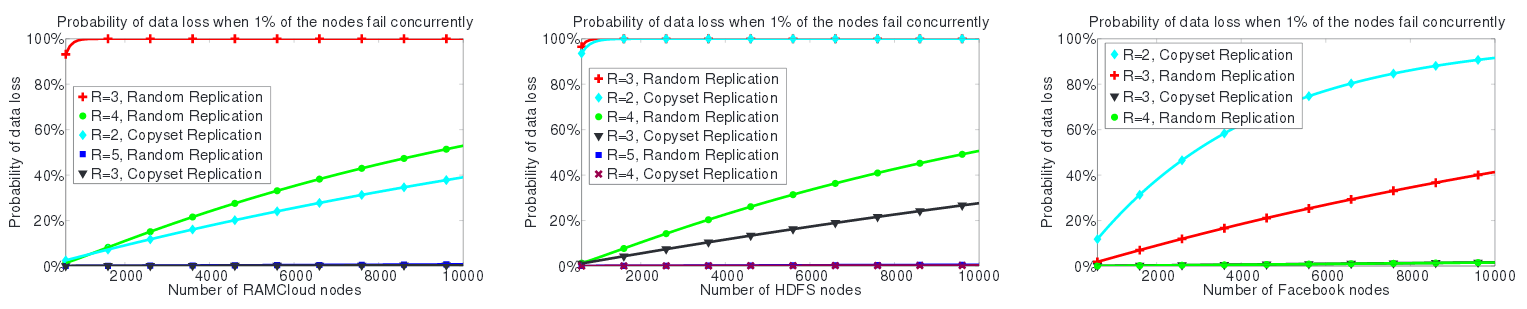
\includegraphics[width=1\textwidth]{7.png}
		\end{figure}
	\end{frame}

	\section{Related Work}

	\begin{frame}
		\frametitle{Related Work}
		\begin{itemize}
			\item BIBD. (Balanced Incomplete Block Designs) $_\text{[Fisher, '40]}$
			\item Power downs. $_\text{[Harnik et al '09, Leverich et al '10, Thereska '11]}$
			\item Multi-fabric interconnects. $_\text{[Mehra, '99]}$
		\end{itemize}
	\end{frame}

	\section{Conclusion}

	\begin{frame}
		\frametitle{Conclusion}
		\begin{enumerate}
			\item Many Storage systems \alert{randomly} spray their data across a large number of nodes.
			\item Serious problem with \alert{correlated failures}.
			\item \alert{Copyset Replication} is a better way of spraying data that \alert{decreases the probability} of correlated failures.
		\end{enumerate}
	\end{frame}

	\begin{frame}
		\frametitle{Thank You for Your Listening}
		\begin{figure}[htb]
			\centering
			\graphicspath{{fig/}}
			
\includegraphics[width=1\textwidth]{8.jpg}
		\end{figure}
	\end{frame}
\end{document}